\documentclass[a4paper]{article}
\usepackage{xgreek}
\usepackage{xltxtra}
\usepackage{setspace}
\usepackage{graphicx}
\newcommand{\HRule}{\rule{\linewidth}{0.5mm}}
\setmainfont[Mapping=TeX-text]{CMU Serif}
\begin{document}
\begin{titlepage}
\begin{center}


\includegraphics[width=0.15\textwidth]{title/Pyrforos2.png}\\[1.cm]
\textsc{\LARGE Εθνικό Μετσόβιο Πολυτεχνείο}\\[1.5cm]

\Large{ Αναφορά Εξαμηνιαίου Project }\\[0.5cm]

% Title
\begin{doublespace}
\HRule \\[0.4cm]
{\huge \bfseries
Βάσεις Δεδομένων
}\\[0.4cm]
Σχεδιασμοί Βάσεων Δεδομένων\\
\end{doublespace}

\HRule \\[1.5cm]

\begin{minipage}{0.4\textwidth}
\begin{flushleft} \large
\begin{tabular}{l l}
Βασίλης \textsc{Γερακάρης} & (08092)\\
Διονύσης \textsc{Ζήνδρος} & (06601)\\
Γρηγόρης \textsc{Λύρας}	& (09687)\\
\end{tabular}
\end{flushleft}
\end{minipage}
\begin{minipage}{0.4\textwidth}
\begin{flushright} \large
\emph{Διδάσκοντες:} \\
Γιάννης \textsc{Βασιλείου}\\
Τίμος \textsc{Σελλής}
\end{flushright}
\end{minipage}

\vfill

{\large \today}
\end{center}
\end{titlepage}

\newcommand{\tab}{\hspace*{3em}}

%{{{ E-R Model
\section{Μοντέλο Οντοτήτων - Συσχετίσεων (ER model)}
Στην εκφώνηση της άσκησης μας δίνονται οι προδιαγραφές μιας βάσης δεδομένων που θα περιέχει
πληροφορίες για το Διεθνή Αερολιμένα Αθηνών Ελευθέριος Βενιζέλος. Με βάση την
περιγραφή αυτή μπορούμε να ορίσουμε τα παρακάτω σύνολα οντοτήτων (entities)
και συσχετίσεων (relations).

\subsection{Οντότητες (entities)}
\begin{itemize}
\item Το αεροπλάνο \emph{(plane)}. Κάθε αεροπλάνο που εξυπηρετείται από τον αερολιμένα.
Προσδιορίζεται από δύο ιδιότητες: το \emph{registration number(αριθμός
εγγραφής)} που έχει το όνομα \emph{pid} στη βάση μας και είναι το πρωτεύον
κλειδί, και τον τύπο του, \emph{tid}, που αποτελεί ξένο κλειδί.
\item Τύπος αεροπλάνου \emph{(type)}. Οι τύποι αεροπλάνων που μπορεί να εξυπηρετήσει το
αεροδρόμιο. Κάθε τύπος έχει ένα \emph{tid} ως πρωτεύον κλειδί, αριθμό επιβατών
\emph{(capacity)}, και το βάρος του \emph{(weight)}.
\item Εργαζόμενος \emph{(employee)}. Κάθε άτομο που εργάζεται στο συγκεκριμένο αεροδρόμιο. Η
οντότητα αυτή έχει ως πρωτεύον κλειδί τον αριθμό μέλους στο εργατικό
σωματείο \emph{(umn)}. Ακόμη έχει αριθμό κοινωνικής ασφάλισης
\emph{(ssn)}, όνομα \emph{(name)}, τηλέφωνο \emph{(phone)},
διεύθυνση \emph{(addr)} και μισθό του εργαζομένου \emph{(salary)} εάν τα γνωρίζουμε.
\begin{itemize}
\item Η οντότητα \emph{employee} είναι υπερτύπος (superclass) των οντοτήτων
\emph{tech} και \emph{regulator}, οι οποίες κληρονομούν τις ιδιότητές
(attributes) της.
\end{itemize}
\item Τύπος ελέγχου \emph{(checktype)}. Πρόκειται για κάθε δυνατό τύπο ελέγχου όπως
ορίζει η FAA. Κάθε τύπος ελέγχου έχει έναν κωδικό αριθμό \emph{(chckid)} που
αποτελεί και πρωτεύον κλειδί ένα όνομα \emph{(name)} και τη μέγιστη δυνατή
βαθμολογία \emph{(maxscore)}.

\pagebreak
Ακολουθούν τα σχήματα οντοτήτων του ER-μοντέλου.
\end{itemize}
\begin{figure}[h]
\centering
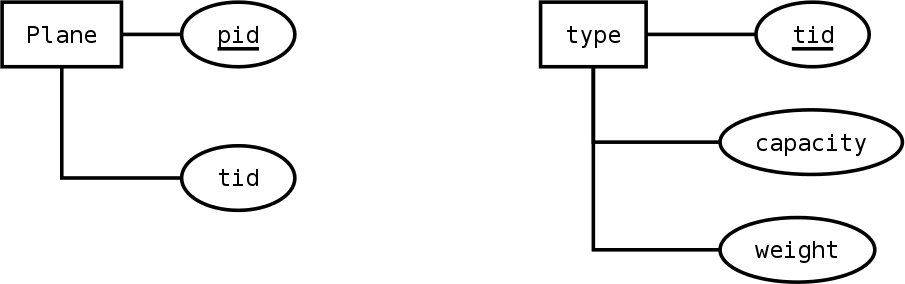
\includegraphics[width=0.85\textwidth]{../ER_model/aviation_entities_a.png}\\
\caption{Οντότητες αεροσκαφών και τύπων.}
\end{figure}
\begin{figure}[h]
\centering
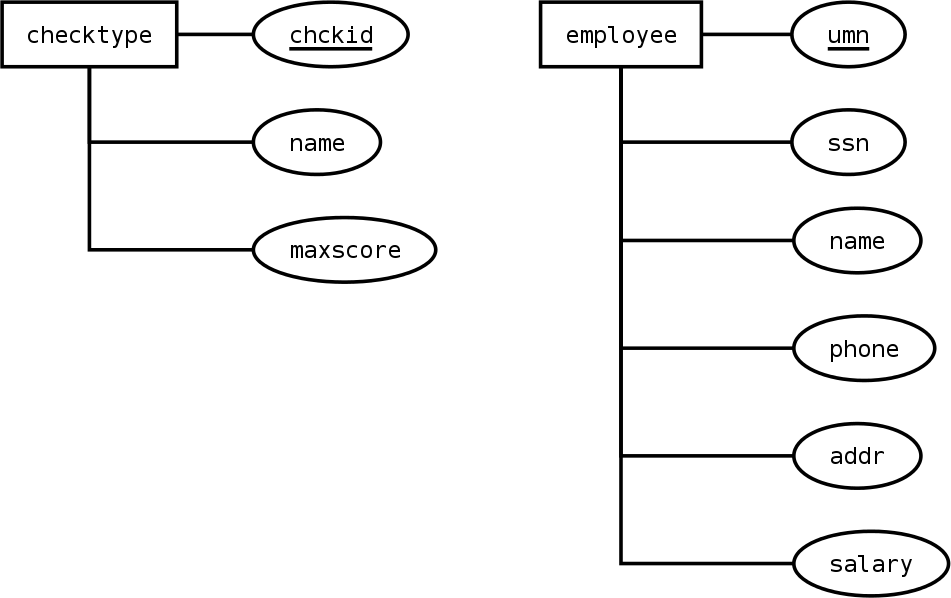
\includegraphics[width=0.85\textwidth]{../ER_model/aviation_entities_b.png}\\
\caption{Οντότητες τύπων ελέγχου και εργαζομένων.}
\end{figure}

\pagebreak
\subsection{Συσχετίσεις (relations)}
\begin{itemize}
\item Η συσχέτιση \emph{ειδικεύεται(specializes)} συνδέει τον κάθε τεχνικό με τον τύπο
αεροπλάνου όπου ο τεχνικός έχει εξειδίκευση. Η συσχέτιση είναι Ν:Μ καθώς ένας
τεχνικός μπορεί να ειδικεύεται σε περισσότερα από ένα αεροσκάφη και πολλοί
τεχνικοί να έχουν ειδίκευση στον ίδιο τύπο αεροσκάφους.
\item Η συσχέτιση \emph{IS\_A} συνδέει τους τεχνικούς και τους ελεγκτές
εναέριας κυκλοφορίας με την οντότητα εργαζόμενος.
\item Η συσχέτιση \emph{ελέγχει(checks)} συνδέει τους τεχνικούς με το αεροπλάνο και τον τύπο
του ελέγχου. Πρόκειται για μια συσχέτιση Ν:Μ:Κ. Πολλοί τεχνικοί μπορούν να
ελέγξουν πολλά αεροσκάφη κάνοντας διαφορετικούς ελέγχους σε κάθε περίπτωση.
\end{itemize}

\begin{figure}[h]
\centering
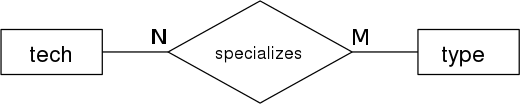
\includegraphics[width=0.7\textwidth]{../ER_model/aviation_relations_1a.png}\\
\caption{Συσχέτιση τεχνικού και τύπου αεροπλάνου}
\end{figure}

\begin{figure}[h]
\centering
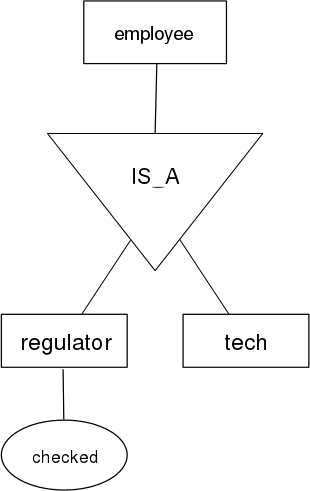
\includegraphics[width=0.5\textwidth]{../ER_model/aviation_relations_1b.png}\\
\caption{Συσχέτιση των τεχνικών και ελεγκτών με τους εργαζόμενους}
\end{figure}

\begin{figure}[h]
\centering
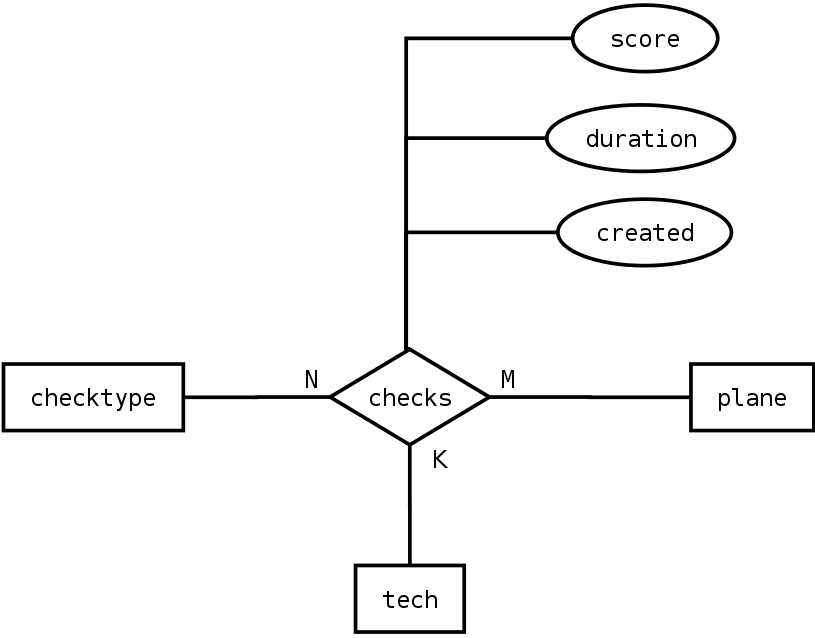
\includegraphics[width=0.9\textwidth]{../ER_model/aviation_relations_2.png}\\
\caption{Συσχέτιση μεταξύ τύπων ελέγχου, τεχνικών και αεροσκαφών}
\end{figure}
\pagebreak
%}}}

%{{{ Relational Model
\section{Σχεσιακό Μοντέλο  (Relational model)}
Θα μετατρέψουμε το προηγούμενο μοντέλο E-R στο αντίστοιχο σχεσιακό σχήμα.
Ακολουθώντας τους κανόνες σχεδίασης, θα σημειώνουμε το πρωτεύων κλειδί
(Primary Key - PK) με  \underline{\textbf{έντονους και υπογραμμισμένους}} χαρακτήρες,
τα υποψήφια κλειδιά (Candidate Keys) μόνο με \textbf{έντονους}
χαρακτήρες ενώ τα ξένα κλειδιά (Foreign Keys - FK) με \textit{πλάγιους} και ένα αστερίσκο (*) μετά
το όνομά τους.\\


\begin{itemize}
\item Οι οντότητες που ορίσαμε στο 1\textsuperscript{o} μέρος της άσκησης
μετατρέπονται απ' ευθείας σε σχέσεις:
\begin{itemize}
\item plane (\underline{\textbf{pid}}, tid)
\item employee (\underline{\textbf{umn}}, \textbf{ssn}, \textbf{name}, phone, addr, salary)
\tab \item tech(\underline{\textit{umn*}})
\tab \item regulator (\underline{\textit{umn*}}, checked)
\item type (\underline{\textbf{tid}}, capacity, weight)
\item checktype (\underline{\textbf{chckid}}, \textbf{name}, maxscore)\\
\end{itemize}

\item Στη συνέχεια μετατρέπουμε τις συσχετίσεις του E-R model σε σχέσεις:
\begin{itemize}
\item checks (\underline{\textit{umn*}, \textit{chckid*}, \textit{pid*}}, created,
duration, score)
\item specializes (\underline{\textit{umn*}, \textit{tid*}})\\

\end{itemize}
\end{itemize}

\begin{itemize}
\renewcommand{\labelitemi}{$\diamondsuit$}
\item Σε όλες μας τις σχέσεις, τα PK είναι αριθμητικά πεδία, γεγονός που
συμβάλλει στην αποδοτικότητα και τη σωστή λειτουργία της βάσης μας.
\item Παρατηρούμε ότι στις συσχετίσεις το PK προκύπτει από την ένωση των
κλειδιών των οντοτήτων που συμμετέχουν σε αυτές.
\item Στο σχεσιακό σχήμα μας δεν υπάρχουν σχέσεις Ν:1, οπότε δεν μπορούμε να
συγχωνεύσουμε κάποιες σχέσεις μεταξύ τους για οικονομία και αναγνωσιμότητα.\\
\renewcommand{\labelitemi}{$\bullet$}
\end{itemize}

Στο σχεσιακό μοντέλο συναντήσαμε το πρόβλημα αδυναμίας απεικόνισης
γενίκευσης οντοτήτων (superclass-subclass) και κάλυψης, όπως συνέβη με την
οντότητα employee που είναι γενίκευση των tech και regulator.

Μας δόθηκε όμως η δυνατότητα να εκφράσουμε περιορισμούς με τη χρήση FK, όπως
γίνονται φανεροί από το διάγραμμα του σχήματος που ακολουθεί.

\begin{figure}[h]
\centering
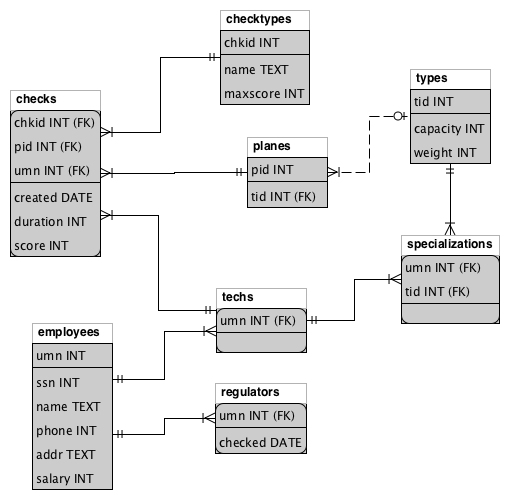
\includegraphics[width=0.9\textwidth]{../R_model/r-db.png}
\caption{Διάγραμμα σχεσιακού μοντέλου}
\end{figure}


%}}}

\end{document}
